\chapter{Astrophysical Processes}
\minitoc
\pagebreak
\section{Quantifying radiation}
\subsection{Flux \& intensity}
Recalling from \textit{Introduction to Astrophysics \& Cosmology} we define the energy flux density (or simply flux), \(F\) as the power per unit surface area.
%
\[ \dd{E} = F \dd{A} \dd{t} \]
%
Note that flux is dependant on the orientation of the unit surface with respect to the Poynting vector of the radiation field.
 Flux has units of J/s/m\(^2\).
 Often it is more useful to use the \emph{monochromatic} energy flux density, \(F_\nu\) where
%
\begin{equation}
	\dd{E} = F_\nu dd{A} \dd{t} \dd{\nu}
	\label{eq:AP:def_flux}
\end{equation}
%
This gives the energy flux per unit of bandwidth, (frequency interval of radiation) which has units J/s/m\(^2\)/Hz.
\par 
In order to account for the differing directions of photons, the flux is further generalised by defining the specific monochromatic intensity, \(I_\nu\).
 This quantifies the power per unit frequency from a range of directions covering a solid angle element \(\dd{\Omega}\) given by
%
\begin{equation}
	\dd{E} = I_\nu \dd{A} \dd{t} \dd{\nu} \dd{\Omega}.
	\label{eq:AP:def_intensity}
\end{equation}
%
This then has units J/s/m\(^2\)/Hz/sr.
 Unlike flux, the intensity is constant along the direction of propagation of photons (in free space).
\par
From the respective definitions, we can relate flux and intensity by
%
\begin{align*}
	F_\nu \dd{A} &= \int \vb{I_\nu} \vdot \vb{\dd{A}} \dd{\Omega}
	\linedrop
	F_\nu \dd{A} &= \int I_\nu \cos(\theta) \dd{A} \dd{\Omega}
	\linedrop
	\therefore F_\nu &= \int I_\nu \cos(\theta) \dd{\Omega}
\end{align*}
%
\subsubsection{Solid angles: an aside}
The solid angle element \(\dd{\Omega}\) is defined
%
\[ \dd{\Omega} = sin(\theta) \dd{\theta} \dd{\phi}, \]
%
hence when integrated over a complete sphere, \(\Omega = 4\pi\)~sr.
 This corresponds to the area of a sphere with unit radius.
 Considering the fraction of the total surface area, \(A\) of a sphere with radius \(R\), we find that
%
\begin{align}
	\frac{A}{4\pi R^2} &= \frac{\Omega}{4\pi}
	\linedrop
	\Omega &= \frac{A}{R^2}.
	\label{eq:AP:solid_angle}
\end{align}
%
As asserted previously, the solid angle corresponds to the area on a sphere with unit radius.
%
\subsubsection{Surface brightness}
Consider an object which a circular region in the sky with radius \(\theta_c\).
 We choose to position this object such that it is located at the pole of the coordinate system.
 This is done for convenience such that the setup is rotationally symmetric in \(\phi\).
 We can then calculate the flux incident on an aperture.
%
\begin{align*}
	F_\nu &= 2\pi I_\nu \int_{0}^{\theta_c}\diff\theta \sin(\theta) \cos(\theta)
	\linedrop
	F_\nu &= \pi I_\nu \sin^2(\theta_c)
\end{align*}
%
For small \(\theta_c\), \(\sin(\theta_c) \simeq \tan(\theta_c) = R/r\) where \(R\) is the object radius and \(r\) is the object-aperture distance, hence
%
\begin{equation}
	F_\nu = \pi I_\nu  \left( \frac{R}{r} \right) ^2 \propto \frac{1}{r^2}.
	\label{eq:AP:flux}
\end{equation}
%
For an isotropically emitting object (such as a star) the flux can be related to the luminosity (total power generated) by
%
\[F = \frac{L}{4\pi r^2}.\]
%
%
%
\section{Radiative transfer}
\subsection{Free space}
We want to know how intensity, \(I_\nu\) changes along the path of the ray.
 Consider two areas placed parallel to each other with a line length \(R\) connecting their centres.
 If the areas are small relative to their separation, then all rays that pass through \emph{both} surfaces are effectively normal to the surfaces.
 From energy conservation,
 %
\begin{align*}
	\dd{E_1} &= \dd{E_2}
	\linedrop
	I_{\nu ,1} \dd{A_1} \dd{t} \dd{\nu_1} \dd{\Omega_1} &= I_{\nu ,2} \dd{A_2} \dd{t} \dd{\nu_2} \dd{\Omega_2} ,	
\end{align*}
%
Since, in free space, the frequency remains constant and using equation \ref{eq:AP:solid_angle}:
%
\begin{align*}
		I_{\nu ,1} \dd{A_1} \frac{\dd{A_2}}{R^2} &= I_{\nu ,2} \dd{A_1} \frac{\dd{A_1}}{R^2}
		\linedrop
		I_{\nu ,1} &= I_{\nu ,2}.
\end{align*}
%
Given that the two surfaces have arbitrary size, we can conclude that in general, intensity is conserved along ray paths in free space.
 This is \emph{not} the case for flux.
 Intensity is conserved since it is defined as `per unit solid angle'.
 Hence, for a distance \(s\) along the path of a ray,
%
\[\dv{I_\nu}{s} = 0.\]
%
This is the equation of radiative transfer in free space.
%
%
\subsection{In a medium}
We now need  to consider emission generated along the line of sight as well as absorption by the medium.
 This can be quantified by the equation of radiative transfer in a medium,
%
\begin{equation}
	\dv{I_\nu}{s} = j_\nu - \alpha_\nu I_\nu,
	\label{eq:AP:radiative_transfer}
\end{equation}
%
where \(j_\nu\) is the \emph{monochromatic emission coefficient} with units J/s/m\(^3\)/Hz/sr, and \(\alpha_\nu\) is the \emph{monochromatic absorption constant} with units m\(^{-1}\).
 It is simple to realise that doubling the intensity passing through a medium would in turn double the intensity absorbed per metre.
 Note that in free space, \(j_\nu = 0\) and \(\alpha_\nu = 0\).
\par
%
\subsubsection{Emission coefficient}
From the definition of intensity given by equation \ref{eq:AP:def_intensity}, but changing \(\dd{E}\) to \(\delta_E\),
%
\begin{align}
	\dv{\delta_E}{s} &= \dv{I_\nu}{s} \dd{A} \dd{t} \dd{\nu} \dd{\Omega}
	\linedrop
	\dv{\delta_E}{s} &= j_\nu \dd{A} \dd{t} \dd{\nu} \dd{\Omega}
	\linedrop
	\therefore \dd{\delta_E} &= j_\nu \dd{V} \dd{t} \dd{\nu} \dd{\Omega}.
	\label{eq:AP:emission_coef}
\end{align}
%
From equation \ref{eq:AP:emission_coef} we can see that \(j_\nu\) corresponds to the amount of energy radiated per unit volume\footnote{Note that \(\dd{V} = \dd{A} \dd{s}\).}, per unit time, per unit solid angle for a frequency interval.
% 
\subsubsection{Absorption constant}
By using similar treatment for the absorption, we find that
%
\begin{align}
		\dv{\delta_E}{s} &= -\alpha_\nu I_\nu  \dd{A} \dd{t} \dd{\nu} \dd{\Omega}
		\linedrop
		\dv{\delta_E}{s} &= -\alpha_\nu \delta_E.
		\label{eq:AP:absorption_const}
\end{align}
%
Equation \ref{eq:AP:absorption_const} implies that \(\alpha_\nu \dd{s}\) represents the fraction of energy that disappears from the radiation field after travelling a length \(\dd{s}\) through the medium.
%  
\subsubsection{Opacity}
Following from the definition in equation \ref{eq:AP:absorption_const}, we now consider a volume of absorbing particles with number density \(n\) and absorption cross section \(\sigma_\nu\).
 Since each particle obscures an area \(\sigma_\nu\), the total area blocked is \(n\sigma_\nu\dd{V}\).
 Also, the fractional area (through which photons flow) that is blocked by absorbers is
%
\[n \sigma_\nu \dv{V}{A} = n \dd{s} \sigma_\nu,\]
%
hence,
% 
\begin{align*}
	\alpha_\nu &= n \sigma_\nu	
	\linedrop
	\alpha_\nu &= \rho \kappa_\nu.
\end{align*}
%
The \emph{opacity coefficient} \(\kappa_\nu\) is defined such that \(\sigma_\nu \propto \kappa_\nu\). Also, \(\kappa_\nu\) has units m\(^2\)/kg.
%
\subsubsection{Optical depth}
A useful quantity to define is optical depth \(\tau_\nu\), which is a re-scaled distance co-ordinate defined by
%
\[\dd{\tau_\nu} \equiv \alpha_\nu \dd{s},\]
%
which provides a more relevant unit to express distance in, rather than metres.
 The total optical depth can then be defined as
%
\[\tau_\nu (s) = \int_{s_0}^{s} \alpha_\nu \dd{s^\prime}.\]
%
The optical depth becomes particularly useful in the case \(j_\nu = 0\).
 In this situation, the equation of radiative transfer (see equation \ref{eq:AP:radiative_transfer}) becomes
%
\[\dd{I_\nu} = - I_\nu \dd{\tau_\nu}.\]
%
This differential equation is easy to solve and we find that
%
\begin{equation}
I_\nu (\tau_\nu) = I_{\nu,0} e^{\tau_\nu}.
\end{equation}
%
\subsubsection{Source function}
Another useful quantity to define is the source function which follows a similar derivation. %REF Draine 7.4
This, along with the definition for optical depth can be used to further generalise the equation of radiative transfer (\ref{eq:AP:radiative_transfer}).
 The source function, \(S_\nu\) is defined as
%
\begin{equation}
	S_\nu \equiv \frac{j_\nu}{\alpha_\nu}.
\end{equation}
%
The radiative transfer equation can now be defined using both \(S_\nu\) and \(\tau_\nu\) as
%
\begin{align*}
	\dd{I_\nu} &= \frac{j_\nu}{\alpha_\nu} \dd{\tau_\nu} - I_\nu \dd{\tau_\nu}
	\linedrop
	\dd{I_\nu} &= S_\nu \dd{\tau_\nu} - I_\nu \dd{\tau_\nu}.
\end{align*}
%
We can then integrate this to obtain the solution by introducing an integration factor \(e^{\tau_\nu}\).
%
\begin{align*}
	\dv{I_\nu}{\tau_\nu} + I_\nu &= S_\nu
	\linedrop
	e^{\tau_\nu} \qty( \dv{I_\nu}{\tau_\nu} + I_\nu ) &= e^{\tau_\nu} S_\nu
	\linedrop
	\text{product rule} \implies 
	\dv{\tau_\nu}( e^{\tau_\nu} I_\nu ) &= e^{\tau_\nu} S_\nu
	\linedrop
	\dd{(e^{\tau_\nu} I_\nu)} &= e^{\tau_\nu} S_\nu \dd{\tau_\nu}
	\linedrop
	\int_{I_\nu (0)}^{e^{\tau_\nu} I_\nu} \dd{(e^{\tau_\nu} I_\nu)} &= \int_{0}^{\tau_\nu} e^{\tau^{\prime}_\nu} S_\nu \dd{\tau^\prime_\nu}
\end{align*}
%
Performing this integration, and then dividing by the introduced factor of \(e^{\tau_\nu}\) gives the general solution to the equation of radiative transfer, shown in equation \ref{eq:AP:radiative_transfer_gen}
%
\begin{equation}
	I_\nu (\tau_\nu) = I_\nu (0) e^{-\tau_\nu} + \int_{0}^{\tau_\nu} e^{-(\tau_\nu - \tau^\prime_\nu)} S_\nu \dd{\tau^\prime_\nu}.
	\label{eq:AP:radiative_transfer_gen}
\end{equation}
%
As we have seen previously, radiation from a background source is attenuated with an exponential factor given by the optical depth.
 The second term in equation \ref{eq:AP:radiative_transfer_gen} is the intensity generated in the medium due to emission.
 It is apparent that any emission produced is also attenuated by the medium between the point of generation of the emission and the observer.
 For constant \(S_\nu\), we find that
%
\begin{equation}
	I_\nu (\tau_\nu) = I_\nu (0) e^{-\tau_\nu} + S_\nu (1 - e^{-\tau_\nu}).
\end{equation}
%
The limit \(\tau_\nu \gg 1\) is the \emph{optically thick} limit, and \(\tau_\nu \ll 1\) is the \emph{optically thin} limit.
%
%
%
\section{Black body radiation}
Radiation is referred to as `thermal' if the spectrum depends \emph{only} on the temperature of the emitting body.
 The spectrum of `non-thermal' radiation however, is affected by other parameters such as chemical composition, or magnetic field strength.
 A perfect absorber in local thermal equilibrium would radiate black body radiation.
 A commonly cited example would be photons escaping through a small hole in a box containing a ``photon gas'' in equilibrium with the box.
 For isotropic radiation, the spectrum is given by the \emph{Planck function} shown in equation \ref{eq:AP:planck_func}
%
\begin{equation}
	I_\nu \equiv B_\nu = \frac{2 h \nu ^3}{c^2} \frac{1}{\exp(\frac{h \nu}{k_B T}) - 1}.
	\label{eq:AP:planck_func}
\end{equation}
%
The Planck curve is monotonic meaning that for a larger \(T\), all points on the curve are higher; the curves do not cross.
%
\subsubsection{Changing variables}
We can express the Planck function in terms of wavelength rather than frequency.
 In order to do this we must follow this procedure:
 consider a frequency interval \((\nu + \dd{\nu})\) and its corresponding wavelength interval \((\lambda + \dd{\lambda})\).
 We require that the intensity should be the same when considering these intervals, i.e.\ \(B_\nu \dd{\nu} \equiv B_\lambda \dd{\lambda}\) hence,
%
\begin{align}
	B_\lambda &= B_\nu \abs{\dv{\nu}{\lambda}}				\nonumber 
	\linedrop
	B_\lambda &= B_\nu \abs{\dv{(c/\lambda)}{\lambda}}		\nonumber
	\linedrop
	B_\lambda &= B_\nu \frac{c}{\lambda^2}					\nonumber
	\linedrop
	B_\lambda &= \frac{c}{\lambda^2} \frac{2 h (c/\lambda)^3}{c^2} \frac{1}{\exp(\frac{h c}{k_B T \lambda}) - 1} \nonumber
	\linedrop
	B_\lambda &= \frac{2 h c^2}{\lambda^5} \frac{1}{\exp(\frac{h c}{k_B T \lambda}) - 1}
\end{align}
%
Note that we use the absolute value of the derivative since both \(\dd{\lambda}\) and \(\dd{\nu}\) were defined to be positive whereas the derivative is negative.            
%
\subsubsection{High and low frequency limits}
The long and short wavelength limits were determined empirically before the theoretical derivation of the Planck function.
\par 
The high frequency (short wavelength) limit where \(h\nu \gg k_B T\) is known as the \emph{Wien} limit.
 The exponential term is much larger than one, hence
%
\begin{equation}
	B_\nu \simeq \frac{2 h \nu^3}{c^2} \exp(\frac{-h\nu}{k_BT}).
	\label{eq:AP:wien_limit}
\end{equation}
%
The low frequency (long wavelength) limit where \(h\nu \ll k_B T\) is known as the \emph{Rayleigh-Jeans} limit.
 In this limit, the exponential term is expanded as \(\exp( h\nu/k_BT) = 1 + h\nu/k_BT + ...\) Hence,
%
\begin{equation}
	B_\nu \simeq \frac{2 \nu ^2 k_B}{c^2} T.
	\label{eq:AP:rayleigh_jeans_limit}
\end{equation}
%
This motivates the common practice in radio astronomy to refer to intensities as `brightness temperatures'.
%
%
\subsection{Kirchhoff's law}
We can relate the Planck function to the source function (\(S_\nu\)).
 Consider an optically thick cloud in thermal equilibrium emitting thermal radiation.
 The radiative transfer equation (\ref{eq:AP:radiative_transfer}) can be written as
%
\[ \dd{I_\nu} = S_\nu \dd{\tau_\nu} - B_\nu \dd{\tau_\nu} = 0. \]
%
Since \( I_\nu = B_\nu \) inside the cloud, this implies that
%
\begin{equation}
	S_\nu \equiv \frac{j_\nu}{\alpha_\nu} = B_\nu.
	\label{eq:AP:kirchhoff's_law}
\end{equation}
%
This is known as \emph{Kirchhoff's law}: the source function of thermal radiation is equal to the Planck fundtion.
 Note that in general, the observed intensity is a combination of the source function as well as the background contribution.
%
%
\subsection{Temperature measurements}
\subsubsection{Brightness temperature}
If we take an intensity measurement at a particular frequency, we can define \emph{brightness temperature}, \(T_b\) such that
%
\begin{equation}
	I_\nu = B_\nu (T_b).
	\label{eq:AP:brightness_temperature}
\end{equation}
%
The brightness temperature corresponds to the temperature at which the Planck function would reproduce the observed flux.
 Only if the radiation is black body does \(T_b\) equal the actual temperature of the source.
%
\subsubsection{Stefan Boltzmann law}
The bolometric flux at the surface of a black body is given by the Stefan Boltzmann law,
%
\begin{equation}
	F_\text{surf} = \sigma_{SB} T^4,
	\label{eq:AP:stefan_boltzmann_law}
\end{equation}
%
where \(\sigma_{SB}\) is the Stefan-Boltzmann constant (\(5.67 \times 10^{-8}\) J/s/m\(^2\)/K\(^4\)).
 Therefore, a unit area of the surface of a black body with uniform temperature radiates a power \(\sigma_{SB} T^4\).
 Hence, a measured intensity (assuming the intermediary medium has no effect) can be related to temperature by
%
\begin{equation}
	\pi I = \sigma_{SB} T^4_{\text{eff}},
	\label{eq:AP:effective_temperature}
\end{equation}
%
where \(T_{\text{eff}}\) is the `effective temperature'. We used equation \ref{eq:AP:flux} in the case that \(\theta_c = \pi / 2 \)to relate the flux to the intensity.
 Again, the effective temperature is only equal to the actual temperature when the object being observed is emitting purely black body radiation.
 Note also, that the size of the object should be known before the effective temperature can be determined.
%
%
\subsection{Wien displacement law}
The peak of the Planck function is temperature dependent and described by the Wien displacement law:
%
\begin{equation}
	h \nu_\text{max} = 2.82144 k_B T,
	k_B T \lambda_\text{max} = 0.201 h c.
	\label{eq:AP:wien_displacement}
\end{equation}
%
This implies that the colour of a black body is determined by its temperature. The \emph{colour temperature} of an object can be determined by finding the ratio of intensities measured at two frequencies. Once again, the colour temperature \emph{only} reflects the real temperature if the emitter is a black body.
%
%
%
\section{The fluid mechanics of shock waves}
\subsection{Fluid mechanics and conservation laws}
In previous chapters (see perhaps \texttt{Properties of Matter} or \texttt{Fluid Mechanics}), we have derived the basic fundamentals of fluid mechanics including the following conservation laws.
%
\subsubsection{Conservation of mass}
The change in mass of a volume element is equal to the difference between the mass flowing into the element and the mass flowing out of the element.
%
\begin{equation}
	\pdv{\rho}{t} + \rho \pdv{v}{x} + v \pdv{\rho}{x} = 0.
	\label{eq:AP:continuity_equation}
\end{equation}
%
The `continuity equation' (\ref{eq:AP:continuity_equation}) above assumes that the total amount of matter remains constant, and that the flow is in the \(x\) direction.
%
\subsubsection{Conservation of momentum}
Here we consider all forces acting on a volume element and assume that they act in the\(x\) direction only.
 These forces include pressure, gravity, magnetic, and other forces.
 Only pressure is considered explicitly, the other forces are quantified with the force \(f\) per unit volume.
%
\begin{equation}
	\rho \pdv{v}{t} + \rho v \pdv{v}{x} = -\pdv{P}{x} + f.
	\label{eq:AP:momentum_conservation}
\end{equation}
%
\subsubsection{Conservation of energy}
The equation of energy conservation includes radiation, heat conduction, and pressure fluctuations.
%
\begin{equation}
	\pdv{t}(\frac{1}{2}\rho v^2 + \frac{P}{\gamma - 1}) + \pdv{x}(\left(v\frac{1}{2}\rho v^2 + \frac{\gamma P}{\gamma - 1}\right)) = -\rho v \pdv{x}\phi + \mathcal{L}
	\label{eq:AP:energy_conservation} %REF Eq. 2.59 of Rosswog & Bruggen
\end{equation}
%
This equation assumes that the fluid is an ideal gas with internal energy \(P/(\gamma -1)\rho\), where \(\gamma\) is the adiabatic index, and \(\phi\) is the potential corresponding to all other forces (except pressure) acting on the fluid.
 Energy losses due to conduction, radiation, etc.\ are quantified by \(\mathcal{L}\) (power/unit volume).
%
\subsubsection{Equation of state}
For an ideal gas, the equation of state is given by
%
\begin{equation}
	P = \sum_{i}n_i k_B T = n k_B T \qquad \qq{(ideal gas).}
	\label{eq:AP:ideal_gas}
\end{equation}
%
Here we assume that the gas is in local thermal equilibrium.
 Each particle species is summed over, however if the gas consists of pure hydrogen then the ideal gas equation becomes \(P = n_H k_B T\), whilst if the gas is fully ionised, \(P = (n_H + n_e)k_B T = 2n_H k_B T\).
\par 
If the gas is adiabatic, then the ideal gas law reduces to
%
\begin{equation}
	P = K \rho^\gamma \qquad \qq{(adiabatic \& ideal),}
	\label{eq:AP:adiabatic_ideal_gas}
\end{equation}
%
where \(K\) is a constant, and \(\gamma\) is the adiabatic index (\(5/3\) for a monatomic gas).
\par 
If the gas is isothermal, then
%
\begin{equation}
	P = K\rho \qquad \qq{(isothermal \& ideal),}
	\label{eq:AP:isothermal_ideal_gas}
\end{equation}
%
since the mass density is proportional to the number density of particles.
 Therefore, an isothermal gas behaves as an adiabatic gas with \(\gamma = 1\).
%
%
\subsection{Shock waves preliminaries}
Shock waves occur when perturbations in a gas propagate faster than the speed of sound of the medium (supersonically).
 They play an important role in astrophysical processes such as star formation, high-velocity stellar winds, AGNs, etc.\
 The shock wave, since it travels supersonically, no longer behaves as a wave and instead gives rise to discontinuities in the gas.
 Shocks often occur when fast moving gas hits an obstacle (or the other way around).
%
\subsubsection{Ram pressure}
Consider a solid object hitting a stationary gas.
 In the frame of the object, gas hits it with a large velocity.
 In this scenario we define `ram pressure' which is related to the transfer of momentum from the gas to the object.
\par 
The amount of mass flow though a surface element \(\dd{A}\) perpendicular to the velocity of the gas flow is given by
%
\[\dd{m} = \rho v \dd{t} \dd{A}.\]
%
Hence, the corresponding momentum flow through the surface is
%
\[\dd{m} v = \rho v^2 \dd{t} \dd{A}.\]
%
Given that \(F = \dv*{p}{t}\) and \(P = \flatfrac{F}(A)\) we can express this in terms of a pressure, with \(\dd{A}\) representing a surface element of the surface of the object.
%
\begin{equation}
	P_\text{ram} = \rho v^2.
	\label{eq:AP:ram_pressure}
\end{equation}
%
\subsubsection{Sound waves \& Mach number}
To begin considering shock waves, we need to first define the speed of sound in a gas.
 The speed of sound in an ideal gas (likely derived previously in the \texttt{Properties of Matter} chapter) is given by
%
\begin{equation}
	c_s = \sqrt{\gamma \frac{P}{\rho}}.
	\label{eq:AP:sound_speed_ideal}
\end{equation}
%
Note that the speed of sound is the propagation velocity with respect to the medium.
\par 
Since the speed of sound is an important natural velocity in a medium, we often express velocities as a fraction of this speed.
 This fraction is called the Mach number, and is defined as
%
\begin{equation}
	\mathcal{M} = \frac{v}{c_s}.
	\label{eq:AP:mach_number}
\end{equation}
%
We can numerically evaluate \(c_s\) for pure hydrogen (assumed to be ideal)
%
\begin{equation}
	c_s = 1.2 \sqrt{\frac{T}{100 \text{K}}} \text{km/s}.
	\label{eq:AP:speed_sound_hydrogen}
\end{equation}
%
For typical ISM temperatures (\(\sim 20 \text{K}\)), \(c_s \simeq 550\)m/s.
 While this is fast in human scales, it is not difficult to produce shocks that exceed this speed in the ISM.
%
\subsubsection{The principles of shock waves}
For normal sound waves, the perturbations are small.
 For large perturbations, the speed of sound can no longer be taken to be constant and will be different in different parts of the wave.
 If we consider adiabatic perturbations (eq. \ref{eq:AP:adiabatic_ideal_gas}), we find that
%
\begin{equation}
	c_s = \sqrt{\gamma \frac{P}{\rho}} \propto \sqrt{\frac{\rho ^ \gamma}{\rho}} = \rho ^{\flatfrac{(\gamma - 1)}{2}}.
	\label{eq:AP:sound_speed_density}
\end{equation}
%
If a strong perturbation (e.g a fast moving piston, see figure \ref{fig:AP:shock_piston}) is produced then it induces an overdensity.
\par
%
\begin{minipage}{0.47\textwidth}
	\begin{figure}[H]
		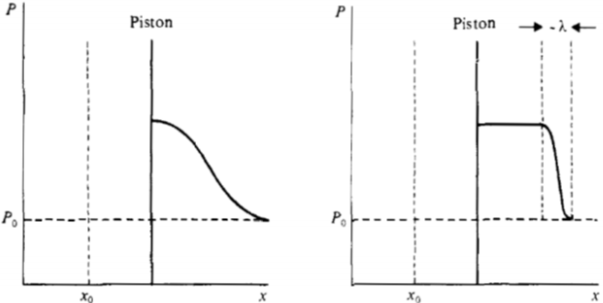
\includegraphics[width = \linewidth]{astro-processes/piston}
		\caption{A graph of pressure against position of the piston.
			 The graph on the right shows the piston after it has been moved rapidly against the gas.}
		\label{fig:AP:shock_piston}
	\end{figure}
\end{minipage}
%
\begin{minipage}{0.47\textwidth}
	The overdensity is greatest near the piston and decays asymptotically to the original density in front of the overdensity.
	 This overdensity travels at the speed of sound which increases with density as shown in equation \ref{eq:AP:sound_speed_density}.
	 As a result, it is inevitable that the overdensity tries to overtake the less dense gas further upstream.
	 This leads to a sharper and sharper front being formed, resulting in, effectively, a discontinuity forming.
	 The thickness of the transition region is determined by the micro-physics, and the mean free path of the particle.
\end{minipage}
%
\par 
In general, the structure of a shock is far more complicated than just a single discontinuity.
 Consider the ejecta of a supernova explosion interacting with the ISM.
 If the ejecta are supersonic, an outer shock will form (known as the `blast wave' of the supernova explosion).
 The outer shock front pushes against the ISM which is accelerated as a result.
 Therefore, on one side of the shock front, the ISM is stationary and not shocked, and on the other side the ISM is shocked and moves in the same direction as the blast wave.
 Since the ISM is being accelerated, the ejecta must be losing kinetic energy; they are being slowed.
 If the shock is strong enough, the deceleration of the ejecta takes place via a \emph{`reverse shock`} (for supernovae) or a \emph{`termination shock`} (for stellar winds).
 Between the two shock fronts, there is a \emph{`contact discontinuity'} (\textbf{not} a shock) where the ISM and ejecta meet.
 In an idealised case, there is no mixing of the two gases, and they are in pressure equilibrium.
\par 
In summary:
%
\begin{itemize}
	\item Unshocked ejecta moves outwards rapidly.
	\item The ejecta pass through the inner shock front, resulting in slower, shocked wind with velocity equal to the shocked ISM on the other side of the contact discontinuity.
	\item The expanding (shocked) ISM is separated from the stationary ISM by the outer shock.
\end{itemize}
%
\subsection{Rankine-Hugeniot jump conditions}
The relationship between the properties of the gas before and after the shock are known as `jump conditions`.
 In the case of an idealised shock with an infinitely thin shock front, the jump conditions are known as `Rankine-Hugeniot conditions'.
\par 
%
\begin{minipage}{0.27\textwidth}
	\begin{figure}[H]
		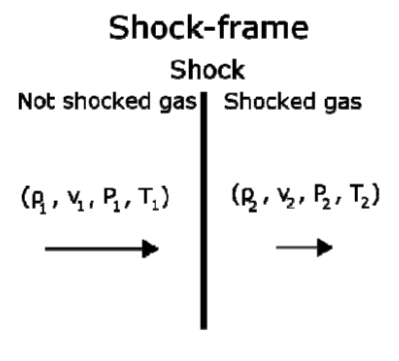
\includegraphics[width = \linewidth]{astro-processes/jump_conditions}
		\caption{Sketch showing the shock in the frame of the shock front.}
		\label{fig:AP:jump_conditions}
	\end{figure}
\end{minipage}
%
\begin{minipage}{0.67\textwidth}
	Since we assumed that the discontinuity is infinitely thin, we can define the pressure, density, and temperature of the unshocked gas to be uniform.
	 By describing the physics in the frame of the shock, there are no explicit time dependencies.
	 In this frame, the unshocked gas moves towards the shock with velocity \(v_1\).
	 After passing the shock front, the gas is perturbed and moves with velocity \(v_2\).
	 Once we have derived the jump conditions, it is easy to consider the same situation from a different frame, for example the frame of the unshocked gas.
	 Although the velocities involved are supersonic, we will assume that the velocities are non-relativistic.
	 The jump conditions are derived from the three conservation laws that were discussed previously.
\end{minipage}
%
\par 

\subsubsection{Mass conservation}
The mass of a unit of gas is conserved across the discontinuity.
 Hence, the amount of mass flowing through a unit area of shock front per unit time is conserved:
%
\[\rho_1 v_1 = \rho_2 v_2 \]
%
This is consistent with equation \ref{eq:AP:continuity_equation} however we must take care of derivatives when discontinuities are involved.
 Noting that there are no explicit time dependencies, we can see that equation \ref{eq:AP:continuity_equation} becomes
%
\begin{align}
	\rho \dv{v}{x} + v \dv{\rho}{x} &= 0	\nonumber
	\linedrop
	\dv{x}(\rho v) &= 0,					\nonumber
	\label{eq:AP:shock_mass_conservation}
\end{align} 
%
hence, writing this as a derivative for a step size of \(\Delta x\) which crosses the discontinuity gives
%
\begin{equation}
	\frac{\rho_2 v_2 - \rho_1 v_1}{\Delta x} = 0.
\end{equation}
%
This equation is satisfied for any arbitrary \(\Delta x\), and confirms the mass conservation condition over the discontinuity that we applied initially.
%
\subsubsection{Momentum conservation}
We also require that momentum is conserved across the discontinuity which is simply given by
%
\begin{equation}
	P_1 + \rho_1 v_1^2 = P_2 + \rho_2 v_2^2.
	\label{eq:AP:shock_momentum_conservation}
\end{equation}
%
\subsubsection{Energy conservation}
Finally, we require energy to be conerved.
 Starting with equation \ref{eq:AP:energy_conservation}, noting that there are no explicit time dependencies, assuming a nonradiative shock (\(\mathcal{L} = 0\)), and assuming that no external forces are present (\( \pdv*{\phi}{x} = 0 \)),
%
\[ \pdv{x}(v \left(\frac{1}{2} \rho v^2 + \frac{\gamma P}{\gamma - 1}\right)) = 0 \]
%
It is immediately apparent that 
\begin{equation}
	\frac{1}{2} v_1^2 + \frac{\gamma}{\gamma - 1 } \frac{P_1}{\rho_1} = \frac{1}{2} v_2^2 + \frac{\gamma}{\gamma - 1 } \frac{P_2}{\rho_2},
	\label{eq:AP:shock_energy_conservation}
\end{equation}
%
where the adiabatic index (\(\gamma\)) is assumed to be constant in the across the shocked and unshocked media.
 The conserved quantity corresponds to the total \emph{specific} (per unit mass) energy of the gas.
%
\subsubsection{Jump conditions in terms of Mach number for a monatomic ideal gas}
The Rankine-Hugeniot jump conditions ensure that mass, momentum, and energy are conserved, hence the following three quantities are conserved over the shock
%
\begin{align}
	\mathcal{F}_\text{mass} &= \rho v,
	\label{eq:AP:shock_mass_conserved}
	\linedrop
	\mathcal{F}_\text{mom} &= P + \rho v^2,
	\label{eq:AP:shock_momentum_conserved}
	\linedrop
	E &= \frac{1}{2}v^2 + \frac{5}{2} \frac{P}{\rho}.
	\label{eq:AP:shock_energy_conserved}
\end{align}
Here we take the adiabatic index \(\gamma = \frac{5}{3}\) which is valid for a monatomic ideal gas.
 We can combine these equations to solve for \(v\).
 First we solve equation \ref{eq:AP:shock_momentum_conserved} for \(\flatfrac{P}{\rho}\), which can be combined with equation \ref{eq:AP:shock_mass_conserved} to give
%
\begin{align}
	\frac{P}{\rho} &= \frac{\mathcal{F}_\text{mom}}{\rho} - v^2 
	\linedrop
	&= \frac{v \mathcal{F}_\text{mom}}{\mathcal{F}_\text{mass}} - v^2
\end{align}
%
We can then substitute this into equation \ref{eq:AP:shock_energy_conserved} to obtain an equation that can be solved for \(v\).







